\documentclass[12pt]{article}
\usepackage[margin=1.5cm]{geometry}
\usepackage{xcolor} % For custom colors
\usepackage{listings}
\usepackage{graphicx}
\graphicspath{ {./images/Lab9} }

% Define SQL style
\lstdefinelanguage{SQL}{
  morekeywords={
    ALTER, ADD, DROP, SELECT, FROM, WHERE, AND, OR, INSERT, INTO, VALUES, UPDATE, SET, DELETE,
    VARCHAR, INT, DATE, FLOAT, BOOLEAN,
    CREATE, TABLE, PRIMARY, KEY, FOREIGN, NOT, NULL, REFERENCES, INNER, OUTER, NATURAL, JOIN, CONSTRAINT,
    LEFT, RIGHT, FULL, ON, AS, USING, DISTINCT, GROUP, BY, ORDER, HAVING, LIMIT, UNIQUE, CASCADE, DEFAULT,
    RENAME, DESCRIBE, TO, IN, IF, CASE, WHEN, THEN, ELSE, END, TIMESTAMPDIFF, CURRENT_DATE, ROUND, CONCAT,
    UNION, WITH, SOME, ALL, EXISTS, ANY, SUM, AVG, COUNT, MIN, MAX, DETERMINISTIC, BEGIN, END, BETWEEN, DECLARE,
    DELIMITER, PROCEDURE, FUNCTION, TRIGGER, BEFORE, AFTER, INOUT, OUT, CALL, FOR, EACH, ROW, RETURN, RETURNS
  },
  sensitive=false,
  morecomment=[l]{--}, % SQL single-line comments
  morecomment=[s]{/*}{*/}, % SQL multi-line comments
  morestring=[b]', % Strings in single quotes
}
\definecolor{darkgreen}{rgb}{0,0.4,0}
\lstset{language=SQL,
    numbers=left,
    basicstyle=\ttfamily,
    showstringspaces=false,
    keywordstyle=\color{blue}\bfseries,
    commentstyle=\color{orange}\itshape,
    stringstyle=\color{darkgreen},
    frame=single,
    breaklines=true
}
    
\begin{document}
\title{CSCD 327 Lab 9}
\author{Dustin Randall}
\maketitle

\section{Find customer's total balance}
\begin{lstlisting}
DELIMITER $
CREATE FUNCTION sumBal(custId INT)
RETURNS DECIMAL(12, 2)
DETERMINISTIC
BEGIN
  DECLARE r DECIMAL(12, 2);
  SELECT SUM(balance) INTO r
  FROM accounts
  WHERE customerID = custId;
  RETURN r;
END $
DELIMITER ;
\end{lstlisting}
\begin{lstlisting}
SELECT customerID, sumBal(customerID) AS totalBalance
FROM customers
WHERE customerID BETWEEN 1 AND 10;
\end{lstlisting}

\begin{figure}[ht]
     \centering
     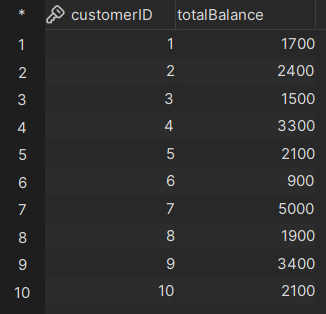
\includegraphics{SumBalance.png}
     \caption{Customer Balances}
 \end{figure}
\pagebreak

\section{Find customer's highest balance}
\begin{lstlisting}
DELIMITER $
CREATE FUNCTION maxBal(custId INT)
RETURNS VARCHAR(50)
DETERMINISTIC
BEGIN
  DECLARE sBal DECIMAL(12, 2);
  DECLARE cBal DECIMAL(12, 2);
  DECLARE r VARCHAR(50);
  
  SELECT balance INTO sBal
  FROM accounts
  WHERE customerID = custId AND accountType='Savings';
  SELECT balance INTO cBal
  FROM accounts
  WHERE customerID = custId AND accountType='Checking';
  
  IF sBal IS NULL AND cBal IS NULL THEN SET r = 'No Account Found';
  ELSEIF sBal IS NULL OR cBal IS NULL THEN SET r = 'One Account Found';
  ELSEIF sBal = cBal THEN SET r = 'Balances Are Equal';
  ELSEIF sBal < cBal THEN SET r = 'Checking Is Greater';
  ELSE SET r = 'Savings Is Greater';
  END IF;
  
  RETURN r;
END $
DELIMITER ;
\end{lstlisting}
\begin{lstlisting}
SELECT customerID, maxBal(customerID) AS msg
FROM customers
WHERE customerID IN(1, 5, 8, 14);
\end{lstlisting}

\begin{figure}[ht]
     \centering
     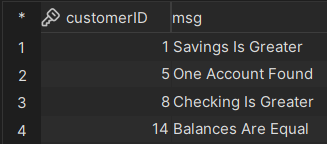
\includegraphics{HighBalance.png}
     \caption{Customer Highest Balances}
 \end{figure}
\pagebreak

\section{Find transaction sums}
\begin{lstlisting}
DELIMITER $
CREATE PROCEDURE sumTrxs(custId INT)
DETERMINISTIC
BEGIN
  SELECT TransactionType, SUM(amount) AS total
  FROM transactions NATURAL JOIN accounts
  WHERE customerID = custId  
  GROUP BY transactionType;
END $
DELIMITER ;
\end{lstlisting}
\begin{lstlisting}
CALL sumTrxs(1);
CALL sumTrxs(5);
CALL sumTrxs(10);
\end{lstlisting}

\begin{figure}[ht]
     \centering
     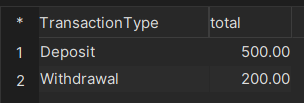
\includegraphics{Trxs1.png}
     \caption{Customer 1}
     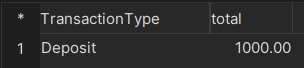
\includegraphics{Trxs2.png}
     \caption{Customer 5}
     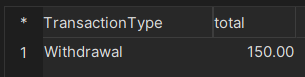
\includegraphics{Trxs3.png}
     \caption{Customer 10}
 \end{figure}
\pagebreak

\section{Make Deposit}
\begin{lstlisting}
DELIMITER $
CREATE TRIGGER applyTrx
AFTER INSERT ON transactions
FOR EACH ROW
BEGIN
  UPDATE accounts
  SET balance = CASE
    WHEN NEW.transactionType = 'Deposit' THEN balance + NEW.amount
    ELSE balance - NEW.amount
    END
  WHERE accountID = new.accountID;
END $
DELIMITER ;
\end{lstlisting}
\begin{lstlisting}
DELIMITER $
CREATE PROCEDURE deposit(acctId INT, amt DECIMAL(12, 2))
DETERMINISTIC
BEGIN
  INSERT INTO transactions(accountID, amount, transactionType, transactionTimestamp)
  VALUES (acctId, amt, 'Deposit', NOW());
END $
DELIMITER ;
\end{lstlisting}

\begin{lstlisting}
SELECT balance FROM accounts WHERE accountID = 1005;
\end{lstlisting}
\begin{figure}[ht]
     \centering
     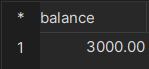
\includegraphics{InitialBal.png}
     \caption{Initial Balance}
 \end{figure}

\begin{lstlisting}
SELECT * FROM transactions WHERE accountID = 1005;
\end{lstlisting}
\begin{figure}[ht]
     \centering
     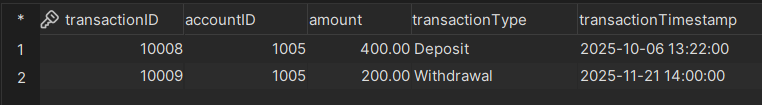
\includegraphics{InitialTrxs.png}
     \caption{Initial Transactions}
 \end{figure}

\begin{lstlisting}
CALL deposit(1005, 100.25);
\end{lstlisting}
\begin{figure}[ht]
     \centering
     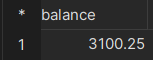
\includegraphics{AfterBal.png}
     \caption{Balance After Deposit}
     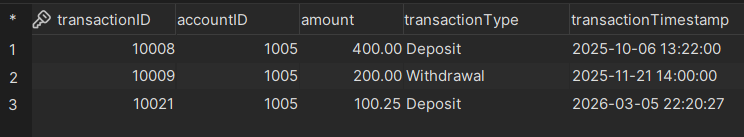
\includegraphics{AfterTrxs.png}
     \caption{Transactions After Deposit}
 \end{figure}
\pagebreak

\section{Make Deposit}
\begin{lstlisting}
DELIMITER $
CREATE PROCEDURE withdrawl(acctId INT, amt DECIMAL(12, 2), OUT msg VARCHAR(20))
DETERMINISTIC
BEGIN
  DECLARE bal DECIMAL(12, 2);
  SELECT balance INTO bal
  FROM accounts WHERE accountId = acctId;
  
  IF amt < bal THEN SET msg = 'Success';
  ELSE SET msg = 'Insufficient Funds';
  END IF;
  
  IF amt < bal THEN
    INSERT INTO transactions(accountID, amount, transactionType, transactionTimestamp)
    VALUES (acctId, amt, 'Withdrawal', NOW());
  END IF;
END $
DELIMITER ;
\end{lstlisting}

\begin{lstlisting}
SELECT balance FROM accounts WHERE accountID = 1001;
\end{lstlisting}
\begin{figure}[ht]
     \centering
     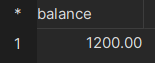
\includegraphics{1001InitialBal.png}
     \caption{Initial Balance 1001}
 \end{figure}

\begin{lstlisting}
SELECT * FROM transactions WHERE accountID = 1001;
\end{lstlisting}
\begin{figure}[ht]
     \centering
     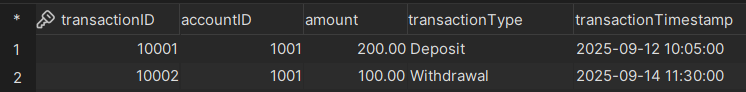
\includegraphics{1001InitialTrxs.png}
     \caption{Initial Transactions 1001}
 \end{figure}

\begin{lstlisting}
SET @msg = '';
CALL withdrawl(1001, 500.75, @msg);
SELECT @msg;
\end{lstlisting}
\begin{figure}[ht]
     \centering
     
\includegraphics{1001Withdrawl.png}
     \caption{Withdrawl message 1001}
     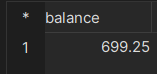
\includegraphics{1001AfterBal.png}
     \caption{Balance after withdrawl 1001}
     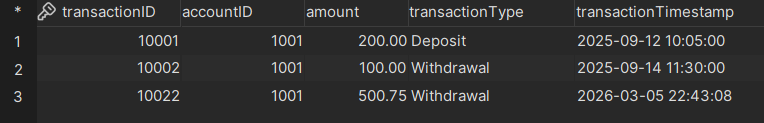
\includegraphics{1001AfterTrxs.png}
     \caption{Transactions After Withdrawal 1001}
\end{figure}

\begin{lstlisting}
SELECT balance FROM accounts WHERE accountID = 1006;
\end{lstlisting}
\begin{figure}[ht]
     \centering
     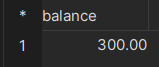
\includegraphics{1006InitialBal.png}
     \caption{Initial Balance 1006}
 \end{figure}

\begin{lstlisting}
SELECT * FROM transactions WHERE accountID = 1006;
\end{lstlisting}
\begin{figure}[ht]
     \centering
     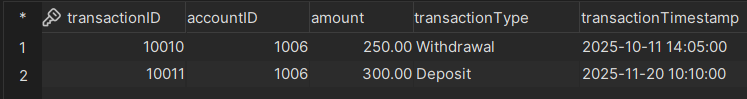
\includegraphics{1006InitialTrxs.png}
     \caption{Initial Transactions 1006}
 \end{figure}

\begin{lstlisting}
SET @msg = '';
CALL withdrawl(1006, 500.75, @msg);
SELECT @msg;
\end{lstlisting}
\begin{figure}[ht]
     \centering
     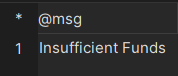
\includegraphics{1006Withdrawl.png}
     \caption{Withdrawl message 1006}
     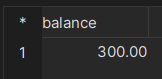
\includegraphics{1006AfterBal.png}
     \caption{Balance after withdrawl 1006}
     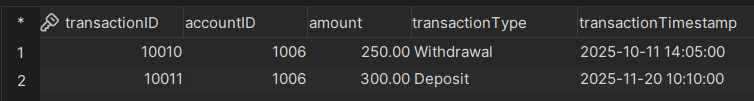
\includegraphics{1006AfterTrxs.png}
     \caption{Transactions After Withdrawal 1006}
\end{figure}
\pagebreak

\section{Transfer Amount}
\begin{lstlisting}
DELIMITER $
CREATE PROCEDURE transfer(cName VARCHAR(40), amt DECIMAL(12, 2), OUT msg VARCHAR(20))
DETERMINISTIC
BEGIN
  DECLARE custId INT;
  DECLARE sId INT;
  DECLARE cId INT;
  DECLARE bal DECIMAL(12, 2);
  
  SELECT customerID INTO custId
  FROM customers WHERE fullName = cName;
  
  SELECT accountID INTO sId
  FROM accounts 
  WHERE accountType = 'Savings'
    AND customerID = custId;
  
  SELECT accountID INTO cId
  FROM accounts
  WHERE accountType = 'Checking'
    AND customerID = custId;
       
  SELECT balance INTO bal
  FROM accounts WHERE accountId = cId;
    
  IF amt <= bal THEN
    BEGIN
    SET msg = 'Success';
    CALL withdrawl(cId, amt, msg);
    CALL deposit(sId, amt);
    END;
  ELSE
    SET msg = 'Insufficient Funds';
  END IF;
END $
DELIMITER ;
\end{lstlisting}
\begin{lstlisting}
SELECT accountType, balance
FROM accounts
WHERE customerID = 
  (SELECT customerID FROM customers WHERE fullName = 'Logan Hall');
\end{lstlisting}

\begin{figure}[ht]
     \centering
     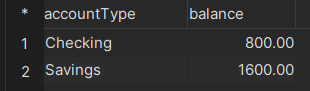
\includegraphics{LoganAccts.png}
     \caption{Logan's Accounts}
 \end{figure}

\begin{lstlisting}
SELECT *
FROM transactions
WHERE accountID IN (
  SELECT accountID FROM accounts
  WHERE customerID = (
    SELECT customerID FROM customers WHERE fullName = 'Logan Hall')
  );
\end{lstlisting}
\begin{figure}[ht]
     \centering
     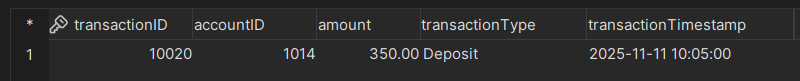
\includegraphics{LoganTrxs.png}
     \caption{Logan's Transactions}
 \end{figure}

\begin{lstlisting}
SET @msg = '';
CALL transfer('Logan Hall', 450.75, @msg);
SELECT @msg;
\end{lstlisting}
\begin{figure}[ht]
     \centering
     
\includegraphics{LoganTransfer.png}
     \caption{Transfer message}
     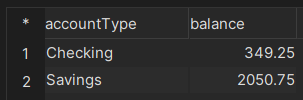
\includegraphics{LoganAfterAccts.png}
     \caption{Logan's Accounts After Transfer}
     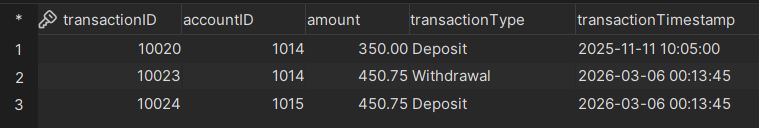
\includegraphics{LoganAfterTrxs.png}
     \caption{Logan's Transactions After Transfer}
 \end{figure}

\begin{lstlisting}
SELECT accountType, balance
FROM accounts
WHERE customerID = 
  (SELECT customerID FROM customers WHERE fullName = 'Sophia Turner');
\end{lstlisting}

\begin{figure}[ht]
     \centering
     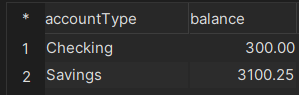
\includegraphics{SophiaInitialAccts.png}
     \caption{Sophia's Accounts}
 \end{figure}

\begin{lstlisting}
SELECT *
FROM transactions
WHERE accountID IN (
  SELECT accountID FROM accounts
  WHERE customerID = (
    SELECT customerID FROM customers WHERE fullName = 'Sophia Turner')
  );
\end{lstlisting}
\begin{figure}[ht]
     \centering
     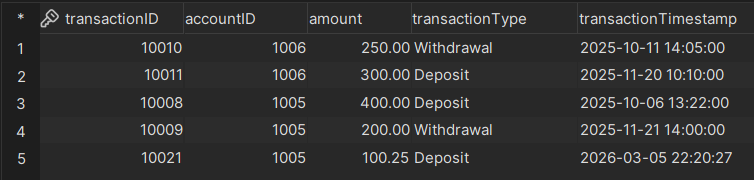
\includegraphics{SophiaInitialTrxs.png}
     \caption{Sophia's Transactions}
 \end{figure}

\begin{lstlisting}
SET @msg = '';
CALL transfer('Sophia Turner', 450.75, @msg);
SELECT @msg;
\end{lstlisting}
\begin{figure}[ht]
     \centering
     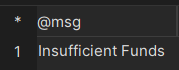
\includegraphics{SophiaTransfer.png}
     \caption{Transfer message}
     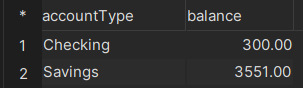
\includegraphics{SophiaAfterBal.png}
     \caption{Sophia's Accounts After Transfer}
     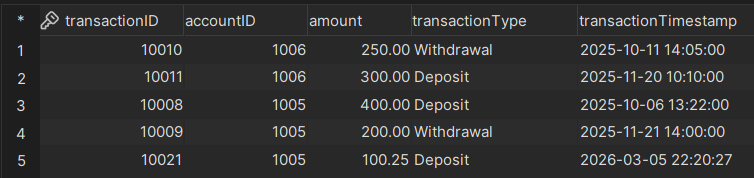
\includegraphics{SophiaAfterTrxs.png}
     \caption{Sophia's Transactions After Transfer}
 \end{figure}

\pagebreak

\end{document}